% It also requires running BibTeX. The commands are as follows:
%
%  1)  latex  aipsamp
%  2)  bibtex aipsamp
%  3)  latex  aipsamp
%  4)  latex  aipsamp
% Use the file aiptemplate.tex as a template for your document.
\documentclass[%
 aip,
%jmp,%
%bmf,%
%sd,%
rsi,%
 amsmath,amssymb,
%preprint,%
 reprint,%
%author-year,%
author-numerical,%
]{revtex4-1}

\usepackage{graphicx}% Include figure files
\usepackage{dcolumn}% Align table columns on decimal point
\usepackage{bm}% bold math
\usepackage{float}
%\usepackage[mathlines]{lineno}% Enable numbering of text and display math
%\linenumbers\relax % Commence numbering lines

\begin{document}

\preprint{AIP/123-QED}

\title[Physics 111B- Hall Effect in a Plasma (HAL) Lab Report]{Hall Effect in a Plasma}


\author{Brandon Tran}
 \email{brandontran7758@berkeley.edu}
\author{Lab Partner: Lok Ching Lui}
\affiliation{$^1$Department of Physics, University of California, Berkeley}


\date{\today}

\begin{abstract}

In this experiment, the Hall Effect is observed in a low-density plasma contained in a discharge tube. Because the density of conduction electrons $n_{e}$ in most laboratory plasmas are many orders of magnitude smaller than in metals, the Hall effect in a plasma is much larger and more easily observable than in metals,\cite{Kunkel}  and thus a quantitative examination of plasma properties is easily obtained. First, the relationship between the discharge voltage and discharge current for a variety of pressures will be determined. Next, a small hysteresis effect is shown to be present through the magnet used in the experiment. The relationship between the Hall field and the applied magnetic field for a variety of pressures will also be determined. From these measurements, the drift velocity, density, collision frequency, average thermal velocity, temperature of the electron gas will be calculated. 

\end{abstract} 

\keywords{plasma, Hall Effect, electron gas, drift velocity, collision frequency, ions}

\maketitle



\section{Introduction}
When a magnetic field is applied perpendicular to an electrical current in a conducting material, a production of a potential difference or Hall voltage arises. The associated Hall field is perpendicular to both the applied magnetic field and current. The Hall field is produced by the Lorentz force which acts on moving charged particles and splits positive and negative charges in opposite directions.\newline
\indent Discovered by Edwin Hall in 1879, the Hall effect allows the sign of charge carriers to be determined and offered the first real proof that electric currents in metals were carried by electrons and not protons. The Hall effect also allows for a quantitative determination of material properties such as the carrier density and mobilities in semiconductors, and has wide-spread applications in devices such as a magnetometers and other types of sensors. \newline
\indent The magnitude of the Hall effect in most metals, however, is very small due to the fact that the Hall field is inversely proportional to the carrier density. The density of conduction electrons in metals is on the order of $10^{29} m^{-3}$, resulting in a very small Hall field. In contrast, most plasmas have carrier densities many orders of magnitude smaller than metals\cite{Kunkel}, and so the Hall effect is much larger and more easily observed. \newline
\indent Section 2 provides a small overview of the theory of the Hall effect and plasma physics, section 3 details the experimental setup and procedure to observe the Hall effect in a plasma, and section 4 contains the main results of the experiment including calculations of the properties of the electron gas.

\section{Theory}
In a normal macroscopic conductor with only one type of carrier present (electrons in this case), the electric current can be described by mobile electron carriers each of charge e and a number density $n_{e}$, which are each moving at a drift velocity $\boldsymbol { u } _ { e }$. The current density $\boldsymbol{j}$ is then

\begin{equation}
\boldsymbol{j} = e n _ { e } \boldsymbol { u } _ { e }
\label{eq:one}
\end{equation}

\noindent The macroscopic current $\boldsymbol { I }$ is then defined as

\begin{equation}
\boldsymbol { I } = \boldsymbol { j } A
\label{eq:two}
\end{equation}

\noindent where A is the cross-sectional area of the conductor. 

\indent In the Hall effect, a potential difference $V _ { \mathrm { H }} $ and therefore a "Hall" field $\boldsymbol { E } _ { \mathrm { H } } $ is induced by moving charges with current $\boldsymbol { I }$ through the Lorentz force on the charges. This Lorentz force $\boldsymbol { F } _ { L }$ is

\begin{equation}
\boldsymbol { F } _ { L } = e \boldsymbol { E } + e \boldsymbol { v } \times \boldsymbol { B } = e \boldsymbol { E } _ { o } + e \boldsymbol { u } _ { e } \times \boldsymbol { B }
\label{eq:three}
\end{equation}

\noindent where $\boldsymbol { B }$ is an externally applied magnetic field which is nonparallel to the current $\boldsymbol { I }$. $\boldsymbol { E } _ { o }$ is often called the "Ohmic" field, and by taking into account the resistivity and therefore the frictional force experienced by these moving charges through the conductor, the Ohmic field can be expressed as 

\begin{equation}
\boldsymbol { E } _ { o } = \eta \boldsymbol { j } = \left( \frac { n _ { e } \nu _ { e } } { m _ { e } e ^ { 2 } } \right) \boldsymbol { j }
\label{eq:four}
\end{equation}

\noindent where $\eta$ is the resistivity of the material, $m _ { e } $ is the mass of the electron, and $\nu _ { e } $ is the collision frequency.
\indent Assuming an applied magnetic field perpendicular to the current $\boldsymbol { I }$ and therefore the Ohmic field $\boldsymbol { E } _ { o }$ by Eq.~(\ref{eq:four}), the Lorentz force induces a "Hall" field $\boldsymbol { E } _ { \mathrm { H } } $ perpendicular to both $\boldsymbol { B }$ and $\boldsymbol { I }$ that exactly cancels the magnetic part of the Lorentz force in Eq.~(\ref{eq:three}). The Hall field can then be defined as 

\begin{equation}
\boldsymbol { E } _ { \mathrm { H } } \cong - \boldsymbol { u } _ { e } \times \boldsymbol { B } = \boldsymbol { B } \times \boldsymbol { j } / e n _ { e }
\label{eq:five}
\end{equation}
\indent In the case of this experiment, the Hall field is indirectly obtained by a measurement of the Hall voltage $V _ { \mathrm { H }} $ produced in a low-density glow discharge column with the current being carried mainly by free electrons. While electrons are produced through ionizing collision with the gas atoms and molecules in the discharge tube, recombination of the charged particles take place almost exclusively at the tube walls.\cite{Kunkel} As a result, the density distribution is not uniform but takes a maximum at the center and falls to zero at the walls as can be seen in Fig.~\ref{fig:density}.

\begin{figure}
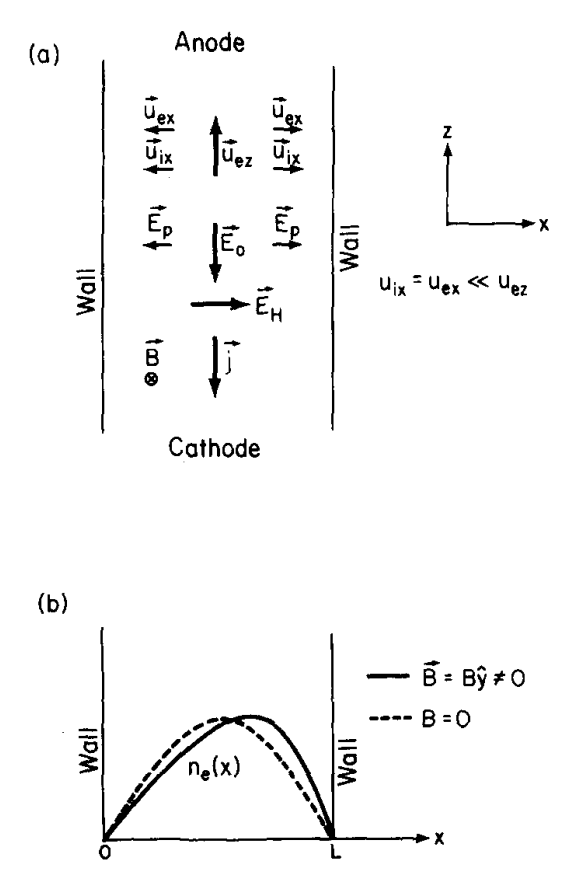
\includegraphics[width=0.6\linewidth]{lateximages/density.png} 
\caption{\label{fig:density} (a) Discharge tube with associated fields $\boldsymbol { B }$, $\boldsymbol { E } _ { \mathrm { H } } $, and $\boldsymbol { E } _ { o }$. (b) electron density of discharge tube in (a) with and without an applied magnetic field. Note the nonuniform density of electrons. (Source: Ref 1)}
\end{figure}

It can then be shown\cite{Kunkel} that the Hall voltage $V _ { \mathrm { H }} $ is

\begin{equation}
V _ { \mathrm { H } } = \int _ { x _ { 1 } } ^ { x _ { 2 } } E _ { x } d x  = \frac { ( x _ { 2 } - x _ { 1 } ) } { 2 } E _ { \mathrm { H } }
\label{eq:six}
\end{equation}

\noindent if we take two points $x _ { 1 }$ and $x _ { 2 }$ symmetrically with respect to the midplane $x=\frac{L}{2}$ as in Fig.~\ref{fig:density}. 


\section{Equipment and Procedure}
The experimental apparatus and setup for this experiment is shown in Fig.~\ref{fig:diagram}. A gas mixture of 98.8$\%$ helium, 1$\%$ argon, and 0.1$\%$ nitrogen is supplied to the discharge tube. The majority of the free electrons in the gas is supplied by the ionized argon, with the nitrogen making the mixture less sensitive to potential contaminations by air and other impurities. 

\begin{figure*}
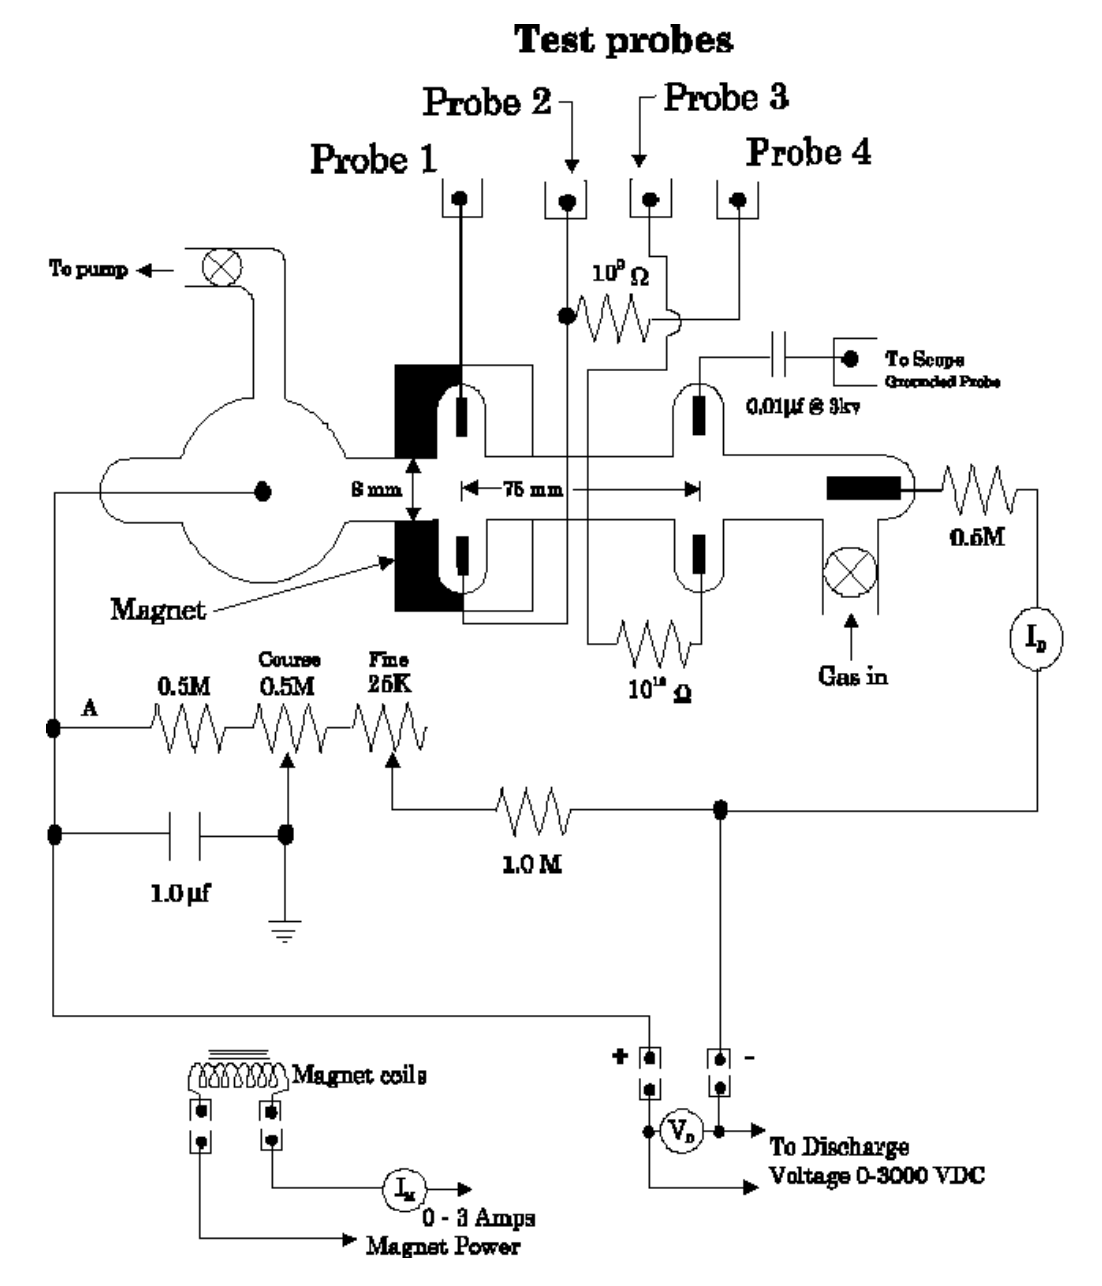
\includegraphics[width=0.5\linewidth]{lateximages/diagram.png} 
\caption{\label{fig:diagram} Experimental setup for the plasma Hall effect experiment. Associated electronic elements like the probes, high voltage supply, and magnet allow measurements of discharge currents and voltages. (Source: Ref 1)}
\end{figure*}

\indent The glow discharge is operated between 15 torr and 30 torr of pressure with discharge currents ranging from 0.2mA and 2.5mA and a high voltage range of 3000V. Because plasmas can support many wave types\cite{Kunkel}, monitoring of fluctuations caused by plasma instabilities, oscillations and striations were achieved by a grounded probe attached to an oscilloscope. Care was taken to prevent oscillations greater than 0.1V for acceptable discharge conditions for data taking. \newline
\indent Using a 0-3000V high voltage supply, a potential difference spanning across 75mm of the tube is supplied. This potential produces a discharge current $\boldsymbol { I}_{d}$ and therefore an Ohmic field $\boldsymbol { E } _ { o }$. $\boldsymbol { E } _ { o }$ accelerates the electrons and causes the free electrons to collide with other gas molecules, ionizing these gas molecules and creating more free electrons and ions. With recombination occurring at the walls, a steady discharge current is established when the frictional force in the gas exactly balances this Ohmic force. Namely, 

\begin{equation}
- m _ { e } \nu _ { e } \boldsymbol{ u } _ { e } = e \boldsymbol { E }_{o}
\label{eq:seven}
\end{equation}

\indent A magnetic field perpendicular to the 8mm diameter of the discharge tube can be applied once this steady discharge current is established, allowing a measurement of the Hall voltage and therefore the Hall field by Eq.~(\ref{eq:six}). Referring to Fig.~\ref{fig:diagram}, the discharge/Ohmic voltage $  V _ { o }$ can be measured between probes 2 and 3 and the Hall voltage $V _ { \mathrm { H }} $ is measured between probes 1 and 2 using a voltmeter. \newline
\indent Again referring to Fig.~\ref{fig:diagram}, the procedure to establish a stable gas flow and pressure in the discharge tube began with a check to make sure all electronics were off and all gas valves closed. The pump was then turned on with the coarse valve open to evacuate any gas occupying the tube. After pressure in the vacuum gauge declined to 2 torr, the main valve on the gas cylinder tank was opened but not yet let into the tube. The coarse valve was then closed and the fine valve open. The gas was then allowed into the tube by adjusting the gas input valve until the pressure rise in the tube was noticeable. The operating pressures in the tube were then adjusted between 15 and 30 torr using the fine valve. \newline
\indent After steady flow was achieved, the high voltage power supply was turned on to about 2500V and the oscilloscope was also turned on to observe fluctuations. The probe circuits were also turned on and adjusted so that probe 2 is referenced to ground (Note each change in conditions required a re-referencing of probe 2 to ground with the potentiometer).

\section{Results and Analysis}
For a variety of pressures between 15 and 30 torr, the discharge voltage $V _ { o }$ was measured as a function of discharge current $\boldsymbol { I}_{d}$ and the magnitude of the Hall field $\boldsymbol { E } _ { H }$ was measured as a function of the magnetic field $\boldsymbol { B }$. The magnetic field was also measured as a function of magnetic current to demonstrate a small hysteresis effect. Using these measurements, a variety of quantitative and illustrative properties of the electron gas were obtained.

\subsection{Discharge Voltage as a function of Discharge Voltage for Varying Discharge Pressures}
The relationship between the discharge voltage $V _ { o }$ vs discharge current $\boldsymbol { I}_{d}$ for pressures ranging from 15 torr to 30 torr in increments of 3 torr are given in Fig.~\ref{fig:VdvsId}. The results show that the discharge voltage is independent of the increasing discharge current at a given pressure. This is in contrast to Ohm's Law (V=IR) in metals, where an increase in current produces a proportional increase in voltage. So unlike conductors, plasmas are nonohmic. There does, however, seem to be a linear relationship between voltage and pressure. With increasing pressure resulting in a proportional increase in discharge voltage. One possible explanation is an increase in pressure results in a higher density of free electrons that are produced, resulting in a higher collision frequency and therefore discharge voltage $V _ { o }$ by Eq.~(\ref{eq:seven}). Note the error bars in the graph were a result of the small plasma oscillations on the oscilloscope and reading errors which contributed to an error of $\pm$2V and $\pm$0.2mA for $V _ { o }$ and $\boldsymbol { I}_{d}$, respectively.

\begin{figure}[H]
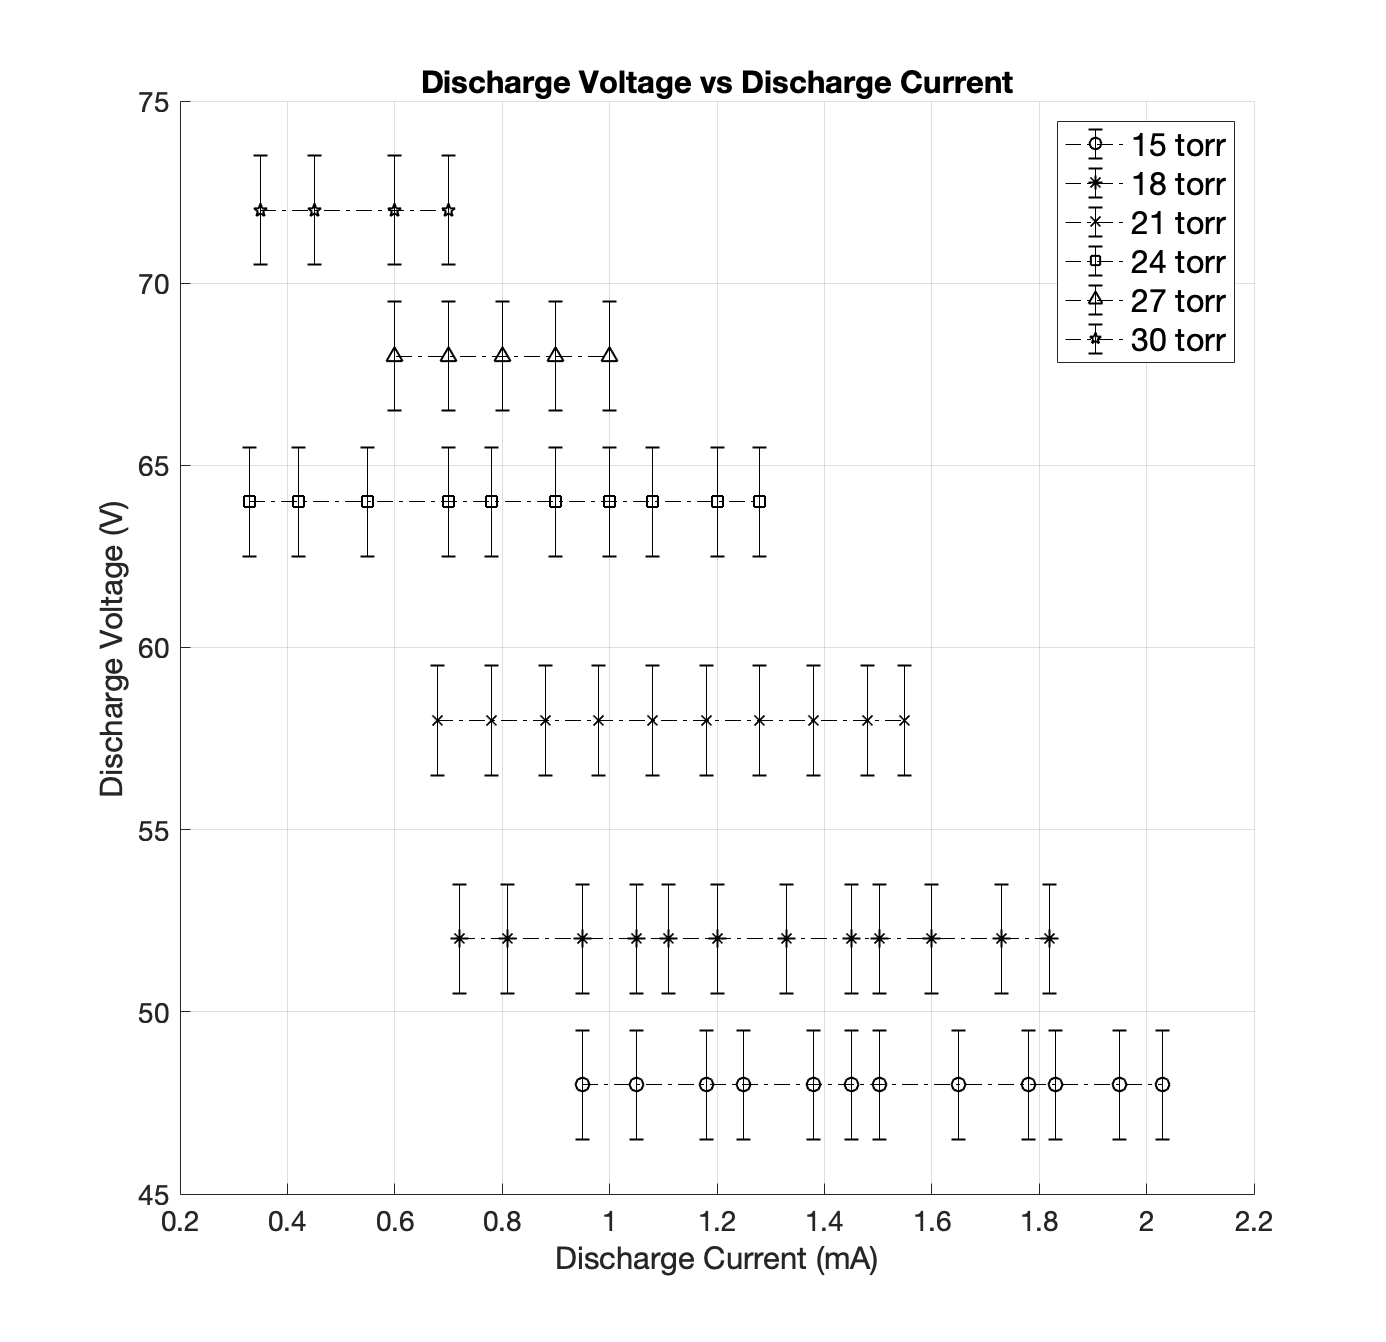
\includegraphics[width=0.965\linewidth]{lateximages/VdvsId.png} 
\caption{\label{fig:VdvsId} Discharge Voltage $V _ { o }$ vs Discharge Current $\boldsymbol { I}_{d}$ for pressures ranging from 15 torr to 30 torr. Instead of an ohmic response expected by Ohm's Law (V=IR), there exists a nonohmic relationship between $V _ { o }$ and $\boldsymbol { I}_{d}$ at a given pressure.  }
\end{figure}

\subsection{Magnetic Field as a function of Magnetic Current}
Next, the magnetic field $\boldsymbol { B }$ was measured as a function of the magnetic current $\boldsymbol { I}_{m}$ using a gaussmeter. The results are shown in Fig.~\ref{fig:MagneticField} below. 


\begin{figure}[H]
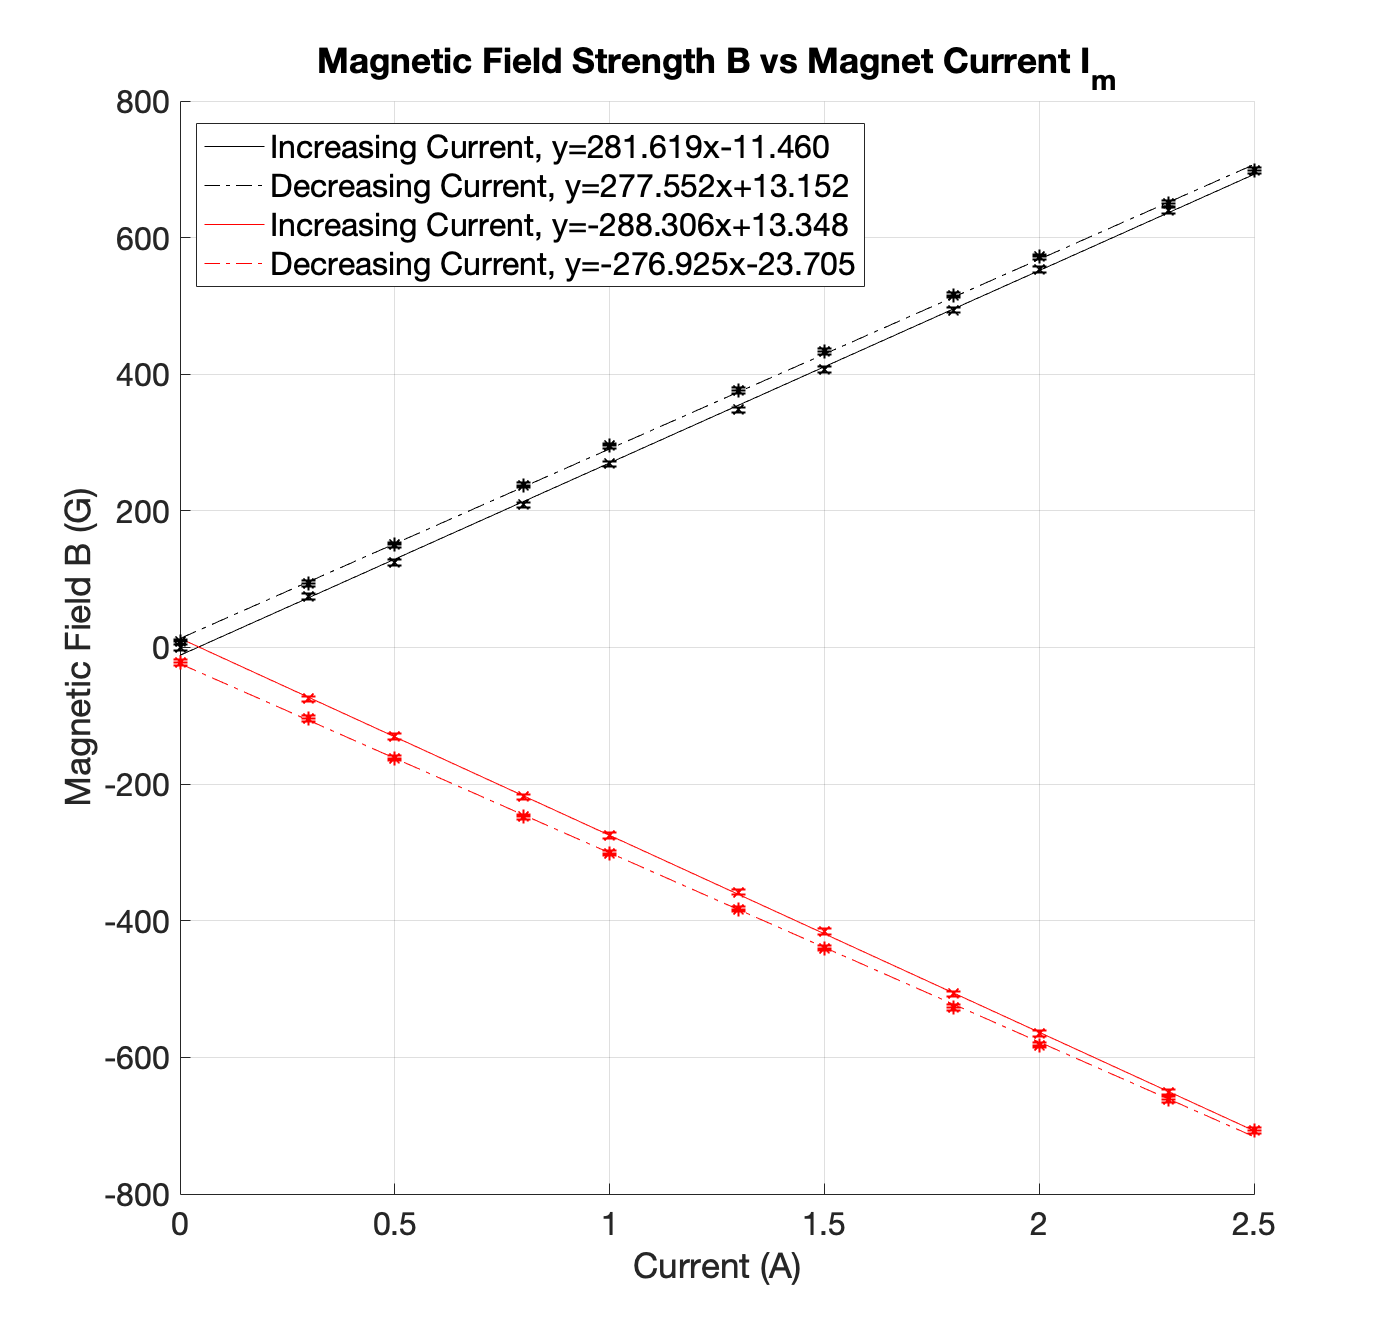
\includegraphics[width=1\linewidth]{lateximages/MagneticField.png} 
\caption{\label{fig:MagneticField} Magnetic Field $\boldsymbol { B }$ as a function of magnet current $\boldsymbol { I}_{m}$. A small hysteresis is evident by the difference in the y-intercept of the second and fourth curves. Note the error bars of approximately 2G resulting from gaussmeter fluctuations are too small to see in the graph. The reduced chi-squared value $\frac{\chi^{2}}{df}$ were 32.11, 20.16, 4.22, and 16.10 for each of the four fits, respectively.}
\end{figure}

The data in black was taken in forward polarity while the red data was taken at reverse polarity. The magnetic field strength was recorded while the magnetic current was first increased at forward polarity and then decreased at the same polarity. The polarity was then reversed with increasing current and then decreasing current. Using a least-squares method, a linear fit was obtained for each curve as shown in the figure. (Note the error bars in the graph were a result of reading errors on the gaussmeter which contributed to an error of $\pm$2G for $\boldsymbol { B }$ ).
 The difference in the y-intercept  for the second and fourth curves was about 37G$\pm$4G, indicating a small hysteresis effect common in ferromagnetic materials such as the one used in this experiment. \newline
\indent Hysteresis arises in a ferromagnetic material when it is magnetized in one direction (by increasing the magnetic current), and does not return to its zero magnetization state once the applied magnetic field is removed (decreasing magnet current to zero). The ferromagnetic core of the magnet used in the experiment can be seen to have hysteresis based on the gaussmeter reading a magnetic field value when the magnet current is 0. This has slight implications for some of the results of the experiment as a magnetic field may be present in the discharge tube when the magnetic current is off. But since this hysteresis effect is small as indicated by the graph, errors associated with them are much smaller than the other errors obtained in this experiment.

\subsection{Hall Field as a function of Magnetic Field for Varying Discharge Pressures}
The Hall voltage $V _ { \mathrm { H } }$ was measured between probes 1 and 2 as a function of the applied magnetic field $\boldsymbol { B }$. The Hall field $\boldsymbol { E } _ { \mathrm { H } }$ is obtained through Eq.~(\ref{eq:six}), with $\frac { ( x _ { 2 } - x _ { 1 } ) } { 2 }=4$ mm, which is the radius of the discharge tube. The Hall field as a function of the magnetic field for six different pressures in increments of 3 torr from 15 torr to 30 torr is shown in Fig.~\ref{fig:HallField} below.

\begin{figure}[H]
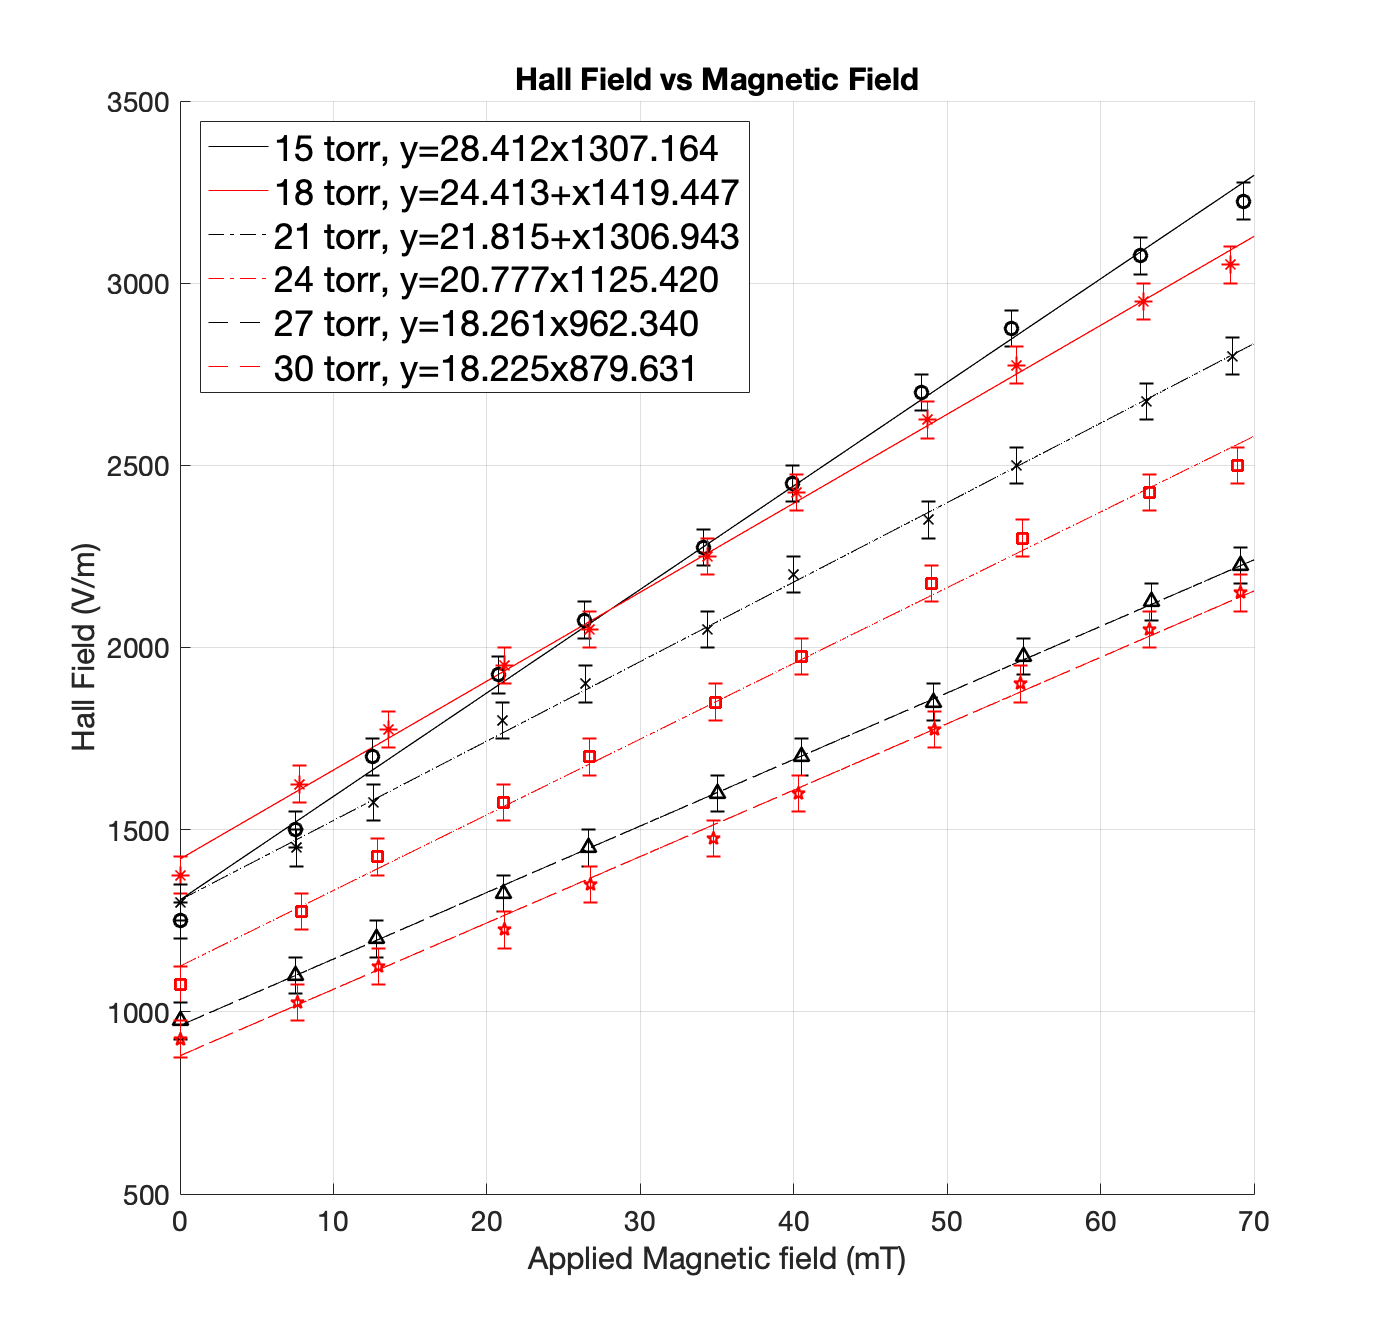
\includegraphics[width=1\linewidth]{lateximages/HallField.png} 
\caption{\label{fig:HallField}  Hall Field $\boldsymbol { E } _ { \mathrm { H } }$ as a function of applied magnetic field $\boldsymbol { B }$ for six different pressures. A linear relationship exists and is expected by Eq.~(\ref{eq:five}). Another general trend that can be seen is at a given magnetic field, the Hall field is lower at higher pressures. This can be seen as the result of the increase in free electrons produced with higher pressures, resulting in lower Hall fields by Eq.~(\ref{eq:five}). Error bars associated with reading errors were approximately $\pm$50V. The reduced chi-squared value $\frac{\chi^{2}}{df}$ for the linear fits were 0.45, 0.30, 0.14, 0.44, 0.04, and 0.30 for 15 torr, 18 torr, 21 torr, 24 torr, 27 torr, and 30 torr respectively.}
\end{figure}

As expected by Eq.~(\ref{eq:five}), a linear relationship between $\boldsymbol { E } _ { \mathrm { H } }$ and $\boldsymbol { B }$ can be seen at each discharge pressure. The least-squares method was applied at each pressure to obtain a linear fit for the data. The equations for the fits are displayed in the legend and the reduced chi-squared values are displayed in the caption of Fig.~\ref{fig:HallField}. (Note the error bars in the graph were a result of reading errors from the voltmeter and plasma oscillations which contributed to an error of $\pm$50V for $\boldsymbol { E } _ { \mathrm { H } }$ and was obtained through a propagation of error on $V _ { \mathrm { H } }$).Another trend that can be seen is for a given applied magnetic field, higher pressures result in lower Hall fields. This further supports the reliability of the data as the Hall field is proportional not only to the applied magnetic field, but also inversely proportional to the electron density by Eq.~(\ref{eq:five}). Higher pressures result in more collisions and more free electrons that are produced, resulting in a higher electron density and therefore a lower Hall field.

\subsection{Calculating Some Properties of the Electron Gas}
Using the data from the Hall field vs magnetic field measurements and also the discharge voltage vs discharge current measurements, a variety of parameters can be calculated for the electron gas in the plasma for varying pressures. In the following sections, the electron drift velocity, electron density, collision frequency, average thermal velocity, and electron temperature will be calculated for the electron gas in the plasma.

\subsubsection{Drift Velocity $\boldsymbol { u } _ { e }$ of Electrons}
By Eq.~(\ref{eq:five}), which states that $\boldsymbol { E } _ { \mathrm { H } } \cong - \boldsymbol { u } _ { e } \times \boldsymbol { B }$, the magnitude of the electron drift velocity is then 


\begin{equation}
u _ { e } = \frac {{ E } _ { \mathrm { H } } } { B }
\label{eq:eight}
\end{equation}

Using this equation and the data from the Hall field vs magnetic field measurements, a plot of the electron drift velocity vs the Hall field for pressures of 15-30 torr were obtained and shown in Fig.~\ref{fig:driftvelocity}. Error bars were calculated using the propagation of error rules on $\boldsymbol { E } _ { \mathrm { H } }$ and $\boldsymbol { B }$. 

\begin{figure}
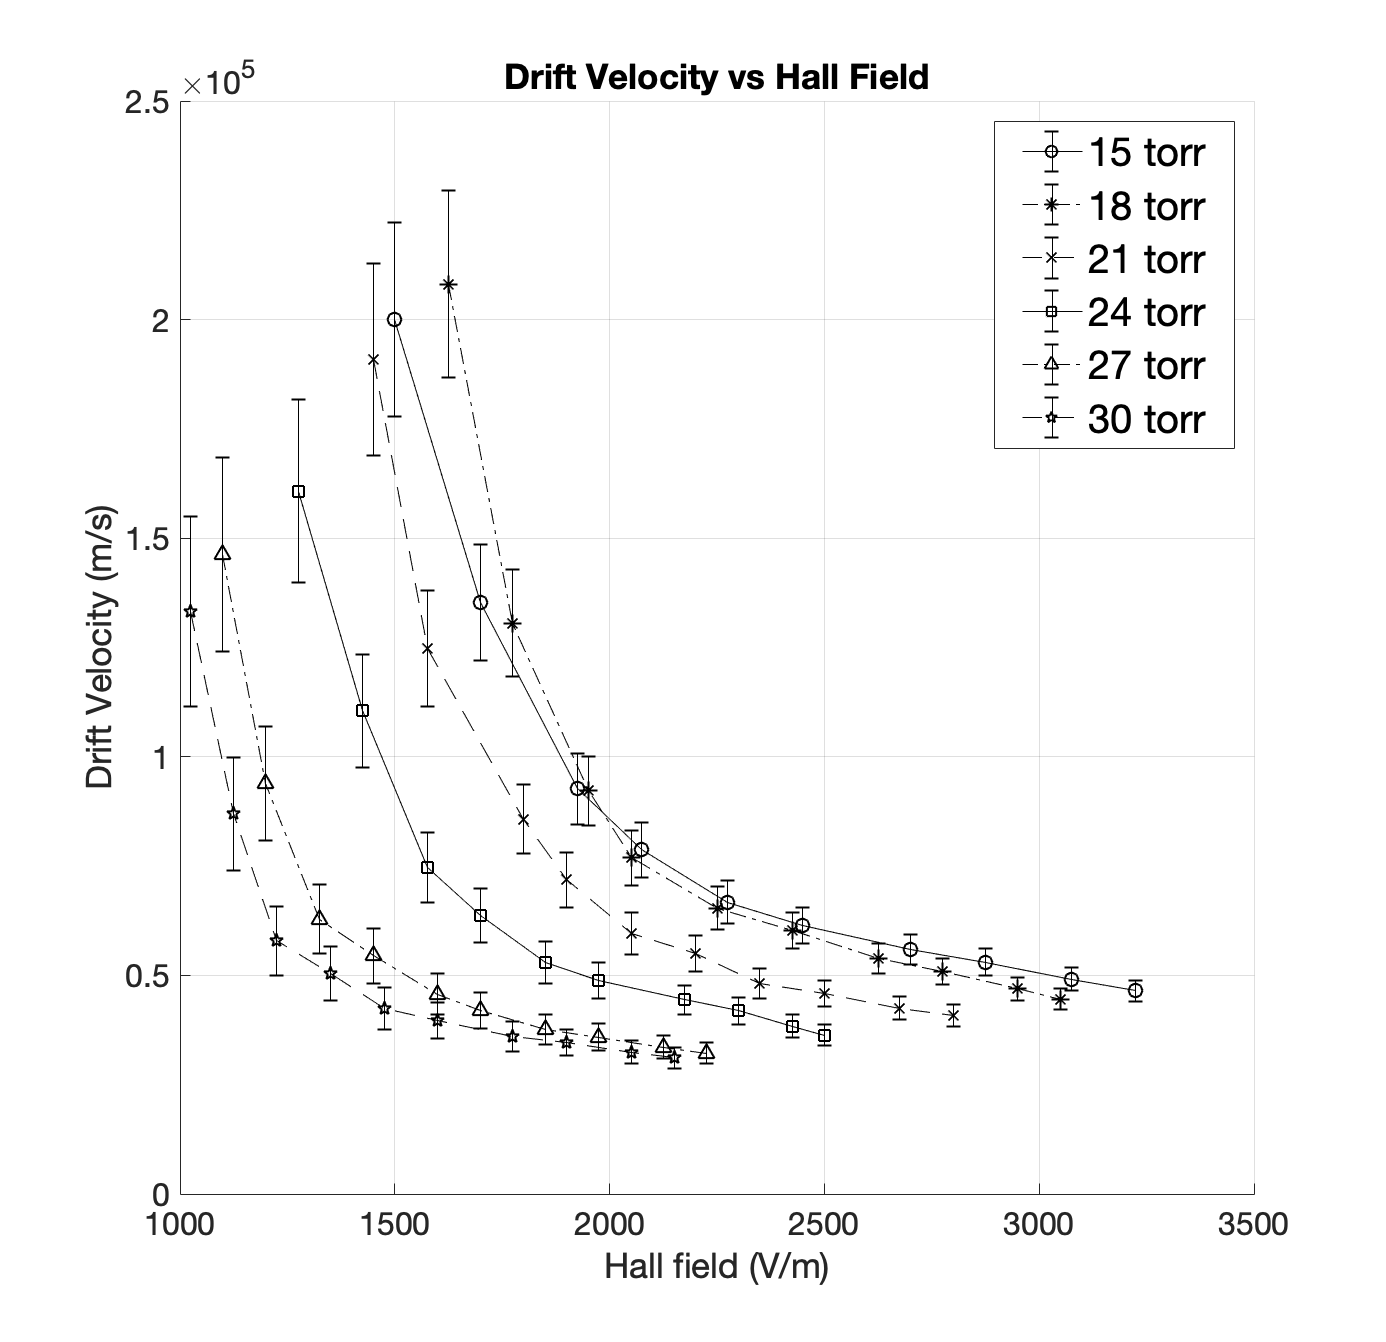
\includegraphics[width=1\linewidth]{lateximages/driftvelocity.png} 
\caption{\label{fig:driftvelocity} Magnitude of the electron drift velocity $u _ { e }$ as a function of Hall field $\boldsymbol { E } _ { \mathrm { H } }$. The drift velocity can be seen to decrease sharply and reaching an asymptotic value with increasing Hall field for a given pressure. For a given Hall field, higher pressures also result in lower drift velocities which can be explained by the increased number of collisions that impede electron motion and therefore reducing drift velocity.}
\end{figure}
A general trend can be seen for each of the six pressures that the electron drift velocity drops steeply with increasing Hall field. All of the electron drift velocities are on the order of $10^5$ m/s and $10^4$ m/s. As a quantitative example, for a pressure of 30 torr and a Hall field of 2000 V/m, the electron drift velocity is approximately 32,000 m/s, which is in good agreement with the typical values obtained in this experiment according to the lab manual. Another trend that can be seen from the graph is that for a given Hall field, higher pressures results in lower drift velocities. This can be explained by the fact that higher pressure results in more collisions, which acts to impede the electron's motion and therefore reducing the drift velocity. \newline
\indent Another thing to note is that the electron drift velocity seems to be reaching an asymptotic value as the Hall field increases for each pressure. This may be accounted for by noting that as the electrons go from one end to the other through the Ohmic force provided by the potential difference between the two ends of the tube, they are also being forced by the Hall field to deflect towards the walls, limiting their minimum drift velocity.

\subsubsection{Electron Density $n_{e}$}
By Eq.~(\ref{eq:one}), $\boldsymbol{j} = e n _ { e } \boldsymbol { u } _ { e }$ and also $\boldsymbol{j}= \frac{\boldsymbol { I }}{A}$ by Eq.~(\ref{eq:two}). Substituting in Eq.~(\ref{eq:two}) for $\boldsymbol{j}$ and Eq.~(\ref{eq:eight}) for $ \boldsymbol { u } _ { e }$ into Eq.~(\ref{eq:one}) and rearranging, the electron density $n _ { e }$ can then be shown to be 


\begin{equation}
n _ { e } = \frac { j } { e u _ { e } }=\frac { I _ { d } B } { e A E _ { \mathrm { H } } }
\label{eq:nine}
\end{equation}

\noindent where A is the cross sectional area of the tube ( $\pi[4mm]^2$ in this case). \newline
\indent Again, using the results of the previous measurements on the Hall field vs magnetic field for a variety of pressures, the electron density was then calculated as a function of the electron drift velocity for six different pressures between 15 torr and 30 torr. The results of these calculations can be seen in the graph of Fig.~\ref{fig:electrondensity}. \newline
\indent As can be seen by the graph, the electron density is inversely related to the electron drift velocity, as expected by Eq.~(\ref{eq:nine}). Higher drift velocities means that electrons are free to flow and are impeded less, which translates to a lower density of electrons to impede flow. It can be also seen that for a given drift velocity, higher pressures result in lower electron densities. This can be explained by referring back to Fig.~\ref{fig:VdvsId}. At higher pressures, discharge currents are lower and since the electron density is proportional to the discharge current, the electron density is also lower. Note error bars were again obtained through propagation of the relevant quantities. \newline
\indent From the graph, the calculated electron densities are on the order of $10^{15}$ electrons/m$^{3}$ at all pressures, which is in good agreement with the example from the lab manual.

\begin{figure}
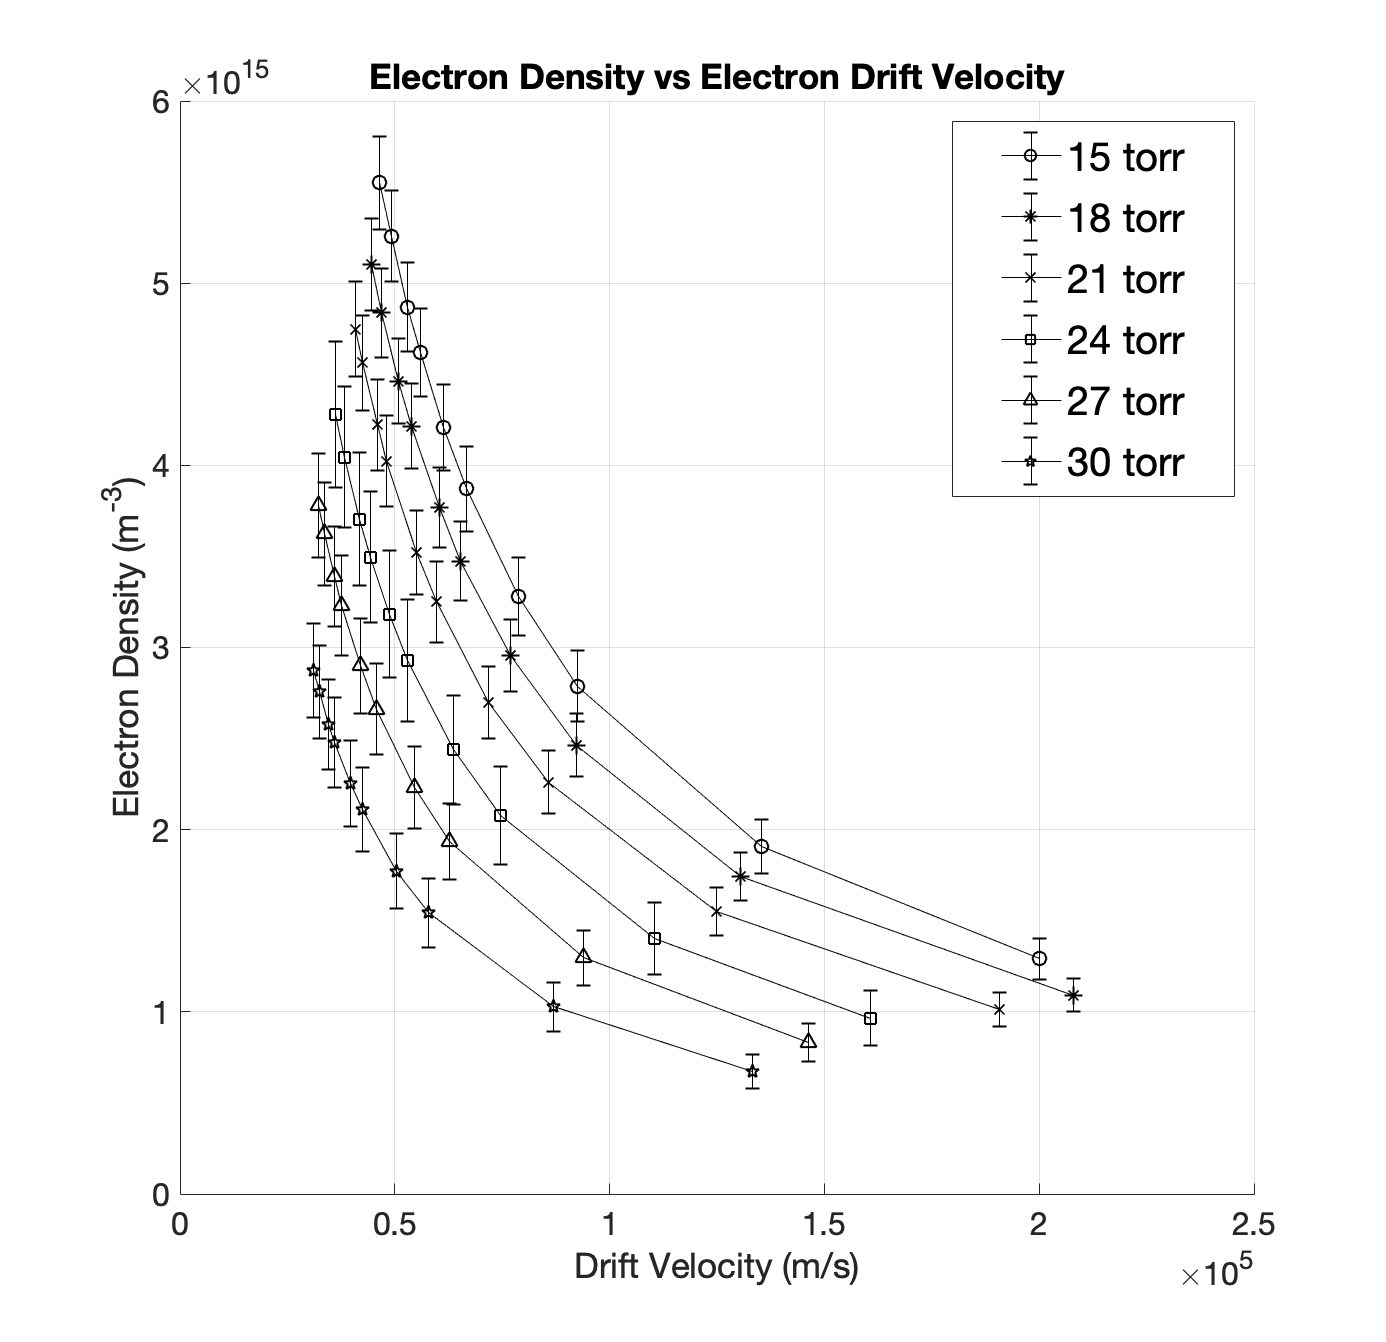
\includegraphics[width=1\linewidth]{lateximages/electrondensity.png} 
\caption{\label{fig:electrondensity} Electron density $n_{e}$ as a function of electron drift velocity $\boldsymbol { u } _ { e }$. As expected by Eq.~(\ref{eq:nine}), higher drift velocities result in lower electron density at a given pressure. Higher pressures also result in lower electron densities as a result of lower discharge currents for a given drift velocity. }
\end{figure}




\subsubsection{Collision Frequency $\nu _ { e }$ of Electrons}
Using Eq.~(\ref{eq:five}) and Eq.~(\ref{eq:seven}), the collision frequency of the electrons can be written as 

\begin{equation}
\nu _ { e } = \left( \frac {  { E } _ { o } } {  { E } _ { \mathrm { H } } } \right) \Omega _ { e }= \frac{e E  _ { o }B}{m_{e}E  _ { H }}
\label{eq:ten}
\end{equation}

The collision frequency of electrons is dependent on three changing parameters in this experiment. Using the same data as before, a plot of collision frequency of electrons $\nu _ { e }$ as a function of the Hall Field ${E}  _ { H }$ was plotted for the six pressures ranging from 15-30 torr. The plot can be seen in Fig.~\ref{fig:collisionfrequency}. Again, the error bars were calculated through propagation of the relevant quantities.

\begin{figure}
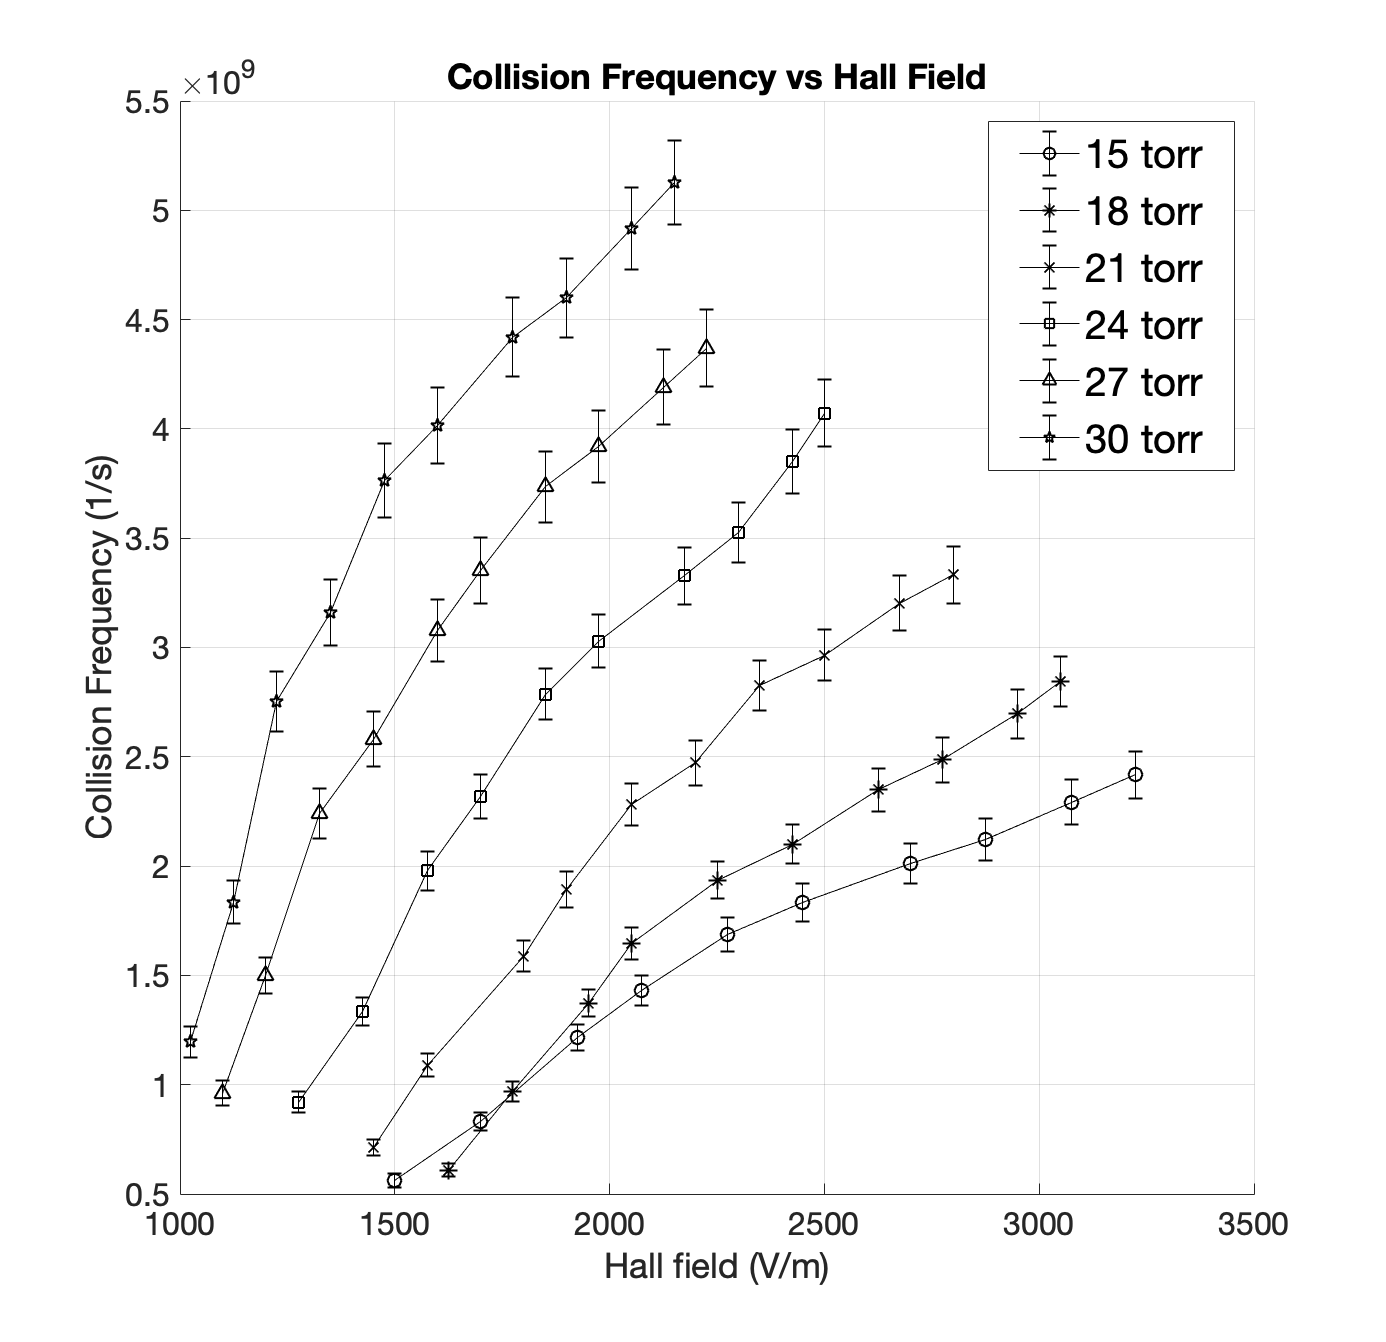
\includegraphics[width=1\linewidth]{lateximages/collisionfrequency.png} 
\caption{\label{fig:collisionfrequency}  Collision frequency of electrons $\nu _ { e }$ as a function of Hall field  ${E}  _ { H }$. Collision Frequency trends upward to an asymptotic value as Hall Field increases due to the magnetic field also increasing. For a given Hall field, higher pressures result in higher electron temperatures that contribute to a higher collision frequency.}
\end{figure}

At first glance, it may seem that the collision frequency dependence on the Hall field is in contrast to Eq.~(\ref{eq:ten}), but the collision frequency is also dependent on the magnetic field $\boldsymbol { B }$ of which the Hall field is also a function of. As the Hall field increases, the applied magnetic field also increases for a given pressure, giving rise to a higher collision frequency. It can be also seen that for a given Hall field, that a higher pressure results in a higher collision frequency, which makes sense as by the ideal gas law pressure is proportional to temperature. And an increase in temperature means an increase in electron collisions. The collision frequency also seems to be reaching an asymptotic value as the Hall field increases, which is in direct agreement with Fig.~\ref{fig:electrondensity}, where the electron density also levels off. Since the collision frequency is also dependent on the electron density, if the electron density levels off to an asymptotic value, so should the collision frequency. \newline
\indent It can be seen from the figure that the collision frequencies at all pressures are on the order of $10^9$ collisions/s. Although there are no numbers for direct comparison to actual experimental values, the results make sense in light of the number density of electrons that are on the order of $10^{15}$ electrons/m$^{3}$ calculated in Fig.~\ref{fig:electrondensity}.

\subsubsection{Average Thermal Velocity $ < | v | > _ { e }$ of Electrons}
Assuming the plasma is a weakly ionized gas, the collision frequency can be written as 

\begin{equation}
\nu _ { e } \cong N _ { g } < \sigma v > _ { e }
\label{eq:eleven}
\end{equation}

\noindent where $< \sigma v > _ { e }$ is the velocity averaged cross-section of the electrons. This assumption is valid because by the ideal gas law $P = N _ { g } k T$, given a room temperature of 295K and a pressure in the middle of the operating pressures, say 24 torr, the number density of the helium atoms $N_{g}$ is approximately $10 ^ { 24 }$ $m ^ { - 3 }$. Also by Fig.~\ref{fig:electrondensity}, the free electron density $n_{e}$ is on the order of $10 ^ { 15 }$ $m ^ { - 3 }$. So the degree of ionization $\frac{n_{e}}{N_{g}}=10 ^ { -9 }$, which verifies the weakly ionized assumption.\newline
\indent Once the velocity averaged cross-section is calculated from the collision frequency results, the average thermal velocity of electrons $ < | v | > _ { e }$ can be written as 

\begin{equation}
< | v | > _ { e } \cong \frac{< \sigma v > _ { e }}{\sigma }
\label{eq:twelve}
\end{equation}

\noindent since $\sigma$ is essentially constant for helium and is approximately $3.8\times 10^{-20}$ $m^{2}$. \newline
\indent Using Eq.~(\ref{eq:eleven}) and Eq.~(\ref{eq:twelve}), the average thermal velocity of the electrons is the plasma gas were calculated as a function of Hall field for six different pressures. The results can be seen in Fig.~\ref{fig:averagevelocity}. Note again error bars were calculated through propagation of relevant quantities. 

\begin{figure}
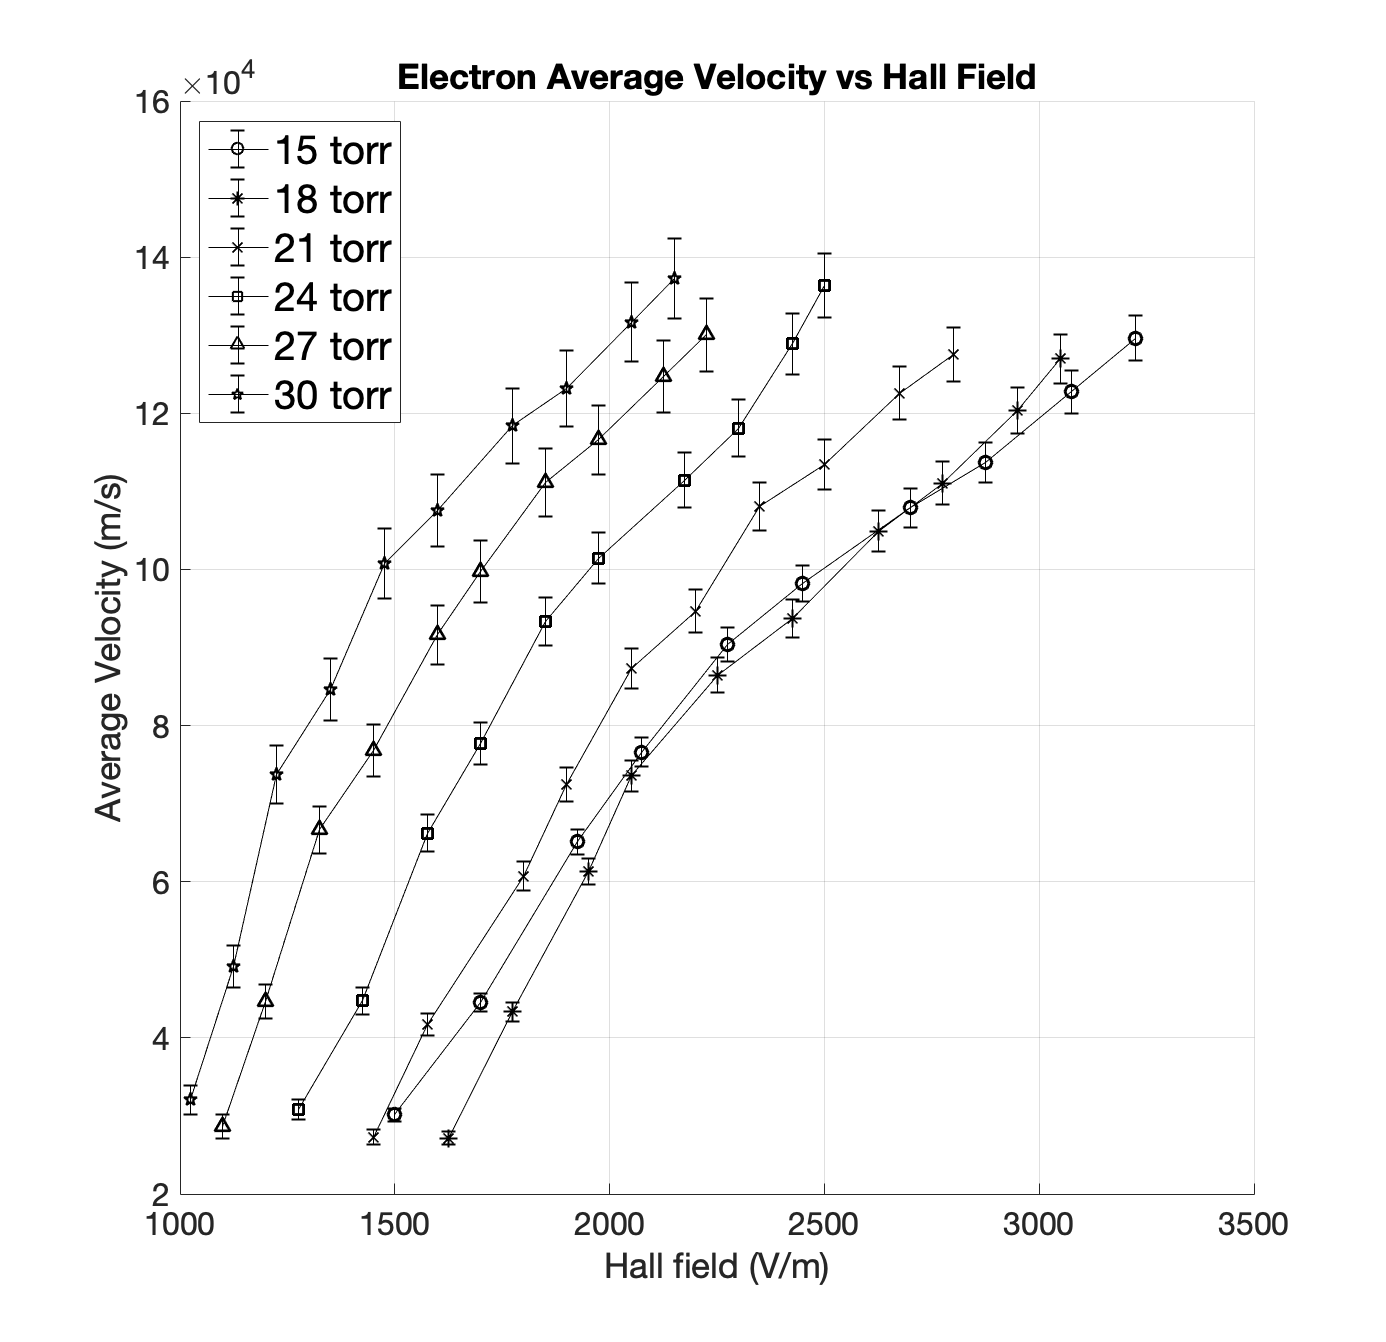
\includegraphics[width=1\linewidth]{lateximages/averagevelocity.png} 
\caption{\label{fig:averagevelocity} Average Thermal Velocity $ < | v | > _ { e }$ of Electrons as a function of Hall field ${E}  _ { H }$. Average velocity increases with Hall field and at higher pressures (with constant Hall field), as expected by an increase in collision frequency in Fig.~\ref{fig:collisionfrequency}.}
\end{figure}

\indent From the graph, it is apparent that the average thermal velocity is on the order of the drift velocities of the electrons that were calculated, which make sense given that they are related by a factor of approximately 1.08 by the Maxwell-Boltzmann distribution. The average velocity also seems to be increasing with Hall field. This is due to the fact that the average thermal velocity is proportional to the collision frequency which is in turn proportional to the Hall field and magnetic field. The average thermal velocity also seems to be increasing with pressure for a given Hall field, which is also in agreement with Fig.~\ref{fig:collisionfrequency}, as the collision frequency also increases with higher pressures.


\subsubsection{Electron Temperatures $T_{e}$}
Lastly, the electron temperatures in the plasma gas can be calculated from a knowledge of the Maxwell-Boltzmann distribution and the average thermal velocity obtained previously. By the Maxwell-Boltzmann distribution, the average thermal velocity $< | v | > _ { e }$ is related to the mean square speed $<  v^2  > _ { e }$ by 

\begin{equation}
<  v^2  > _ { e }=\frac{3\pi}{8}< | v | > _ { e }^2
\label{eq:thirteen}
\end{equation}

And the mean square speed of the electrons is related to the electron temperature by 

\begin{equation}
E _ { e } = \frac { 1 } { 2 } m _ { e } < v _ { e } ^ { 2 } > = \frac { 3 } { 2 } k T _ { e }
\label{eq:fourteen}
\end{equation}

Using Eq.~(\ref{eq:thirteen}) and Eq.~(\ref{eq:fourteen}), along with the calculations of the average thermal velocity, the electron temperatures of the electron gas in the plasma were calculated as a function of Hall field for six different pressures along with a calculation of the mean electron energy as a function of Hall field. The results can be seen in Fig.~\ref{fig:electrontemperature}. Note again error bars were calculated through propagation of relevant quantities. \newline
\indent From the graph, it can be seen that the electron temperatures increase with Hall field at all pressures, which makes sense given that the average velocity also increases at higher Hall fields. At a given Hall field, the electron temperature also increases with higher pressures. A result that can be resolved by referring back to the ideal gas law. \newline
\noindent The electron temperatures mainly lie in the couple of thousand Kelvin range, which is about a factor of 3 or 4 lower than expected. Also, note that the electron temperatures in the plasma are much higher than the ion temperatures (which are about room temperature). The reason the tube does not feel warm to the touch is due to the inefficiency of energy transfer between two bodies of different masses. Electrons are much smaller in mass than their ionic counterparts, meaning they do not transfer energy efficiently to the tube walls and other ions to equilibriate the temperature in the tube in the time observed. 

\begin{figure*}
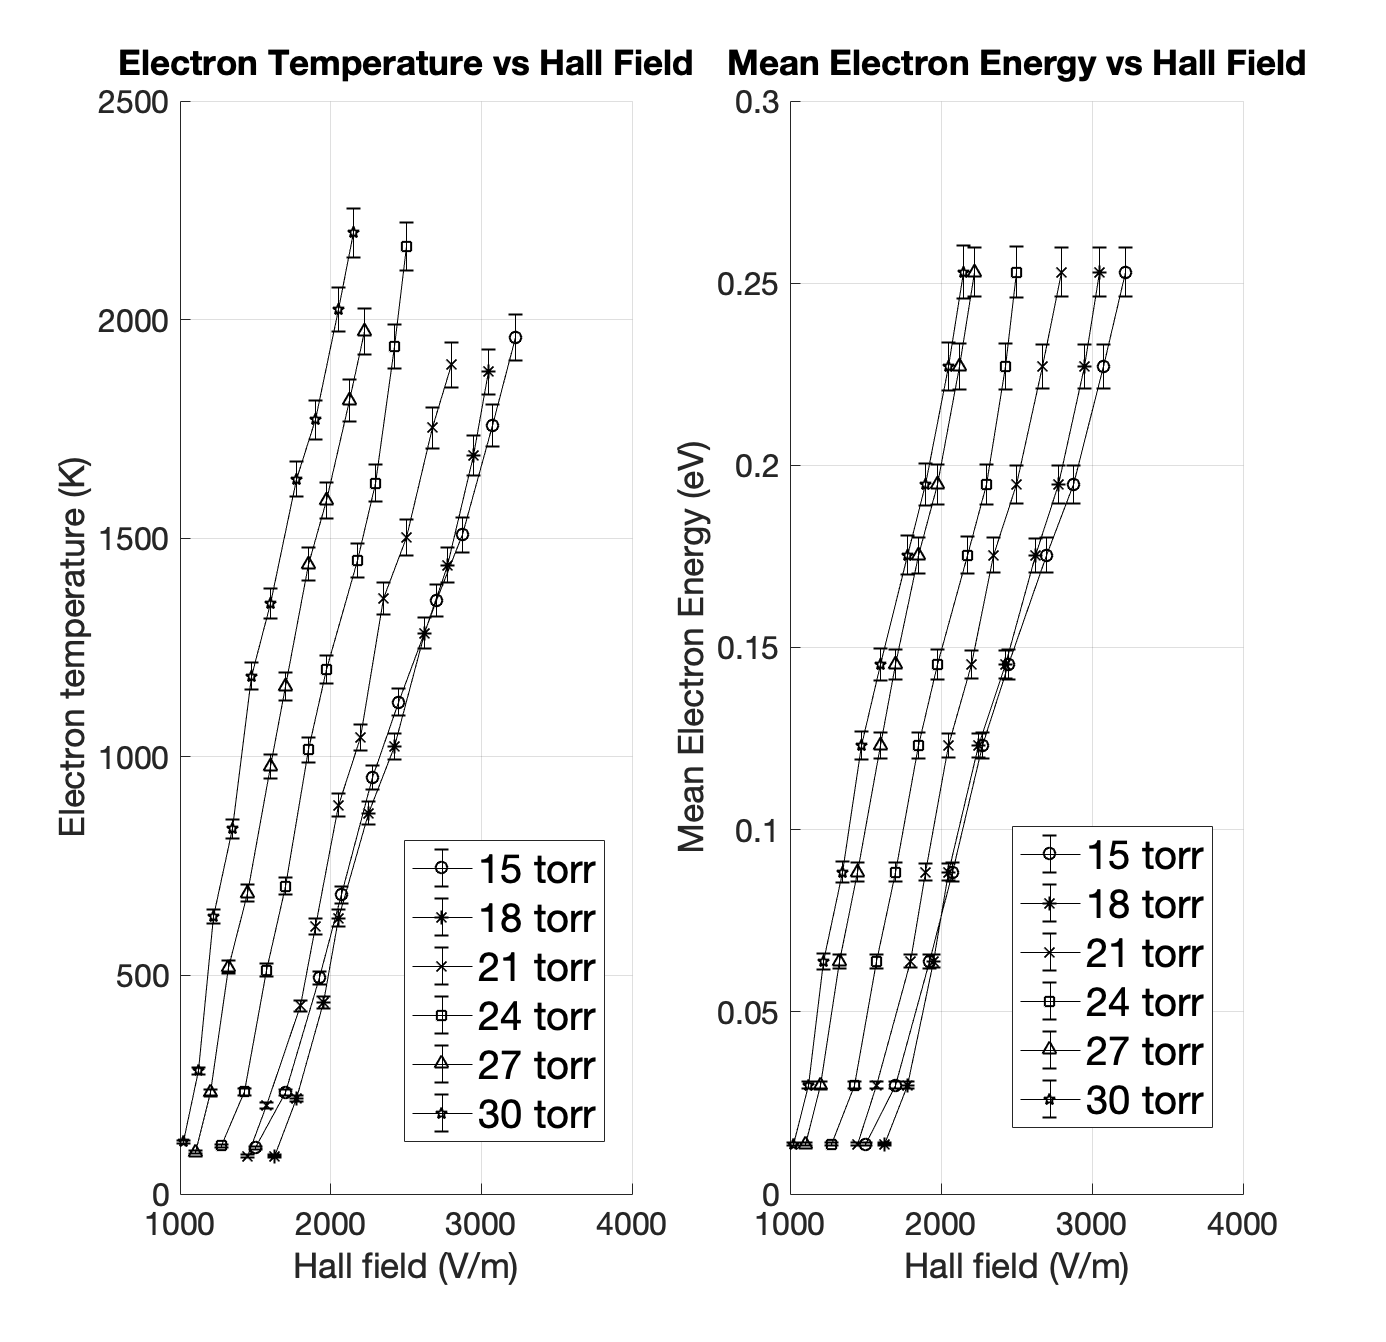
\includegraphics[width=0.8\linewidth]{lateximages/electrontemperature.png} 
\caption{\label{fig:electrontemperature} Electron temperature $T_{e}$ and mean electron energy as a function of Hall field ${E}  _ { H }$. Both quantities increase with Hall field as a result of the increase in average thermal velocity and increase as a function of pressure (at constant Hall field) as a result of the ideal gas law. }
\end{figure*}

\indent Also the second graph in Fig.~\ref{fig:electrontemperature} displays the mean electron energies as a function of Hall field. Again, the mean electron energy is about a factor of 4 lower than expected, but referring back to the Maxwell-Boltzmann distribution, ionization of gas molecules in the tube can still take place even with low mean electron energies due to the fact electron energies follow the distribution. Although the mean electron energy is low, there are a small number of electrons that have a higher energy sufficient to ionize the atoms in the gas, creating what is called an electron avalanche to create a plasma.



\section{Conclusion}
In conclusion, observing the Hall effect in a plasma allowed for certain conclusions to be drawn. The discharge voltage was found to be independent of discharge current at all pressures, to within error, contrasting the typical Ohmic behavior of metals. The Hall field was found to linearly increase with the applied magnetic field, a result expected by Eq.~(\ref{eq:five}). \newline
\indent Using these results, a determination of some quantities of the electron gas in the plasma were also calculated. The drift velocity of the electrons were found to be on the order of $10^5$ m/s and $10^4$ m/s. The electron density was found to be on the order of $10^{15}$ electrons/m$^{3}$. Both quantities were found to be in good agreement with theoretical values. The collision frequency and average thermal velocity of electrons were also calculated to determine the electron temperatures. The collision frequency was on the order of $10^9$ collisions/s while the average thermal velocity was on the order of $10^5$ m/s. The electron temperature was about a factor of 4 lower than expected, but the velocity distribution of the electrons determined by the Maxwell-Boltzmann distribution still allows for sufficiently enough energetic electrons to ionize the gas.  In addition, all of these results were also illustrated through simple thermal physics to have dependences on pressure as can be seen in the graphs.\newline
\indent Although this experiment provided a wealth of information about the plasma and the electron gas, many questions still remain as prompted by these results and a more thoughtful investigation is needed to fully understand the implications of these results.


\begin{acknowledgments}
We would like to thank the Physics 111B staff for their patience and guidance during this experiment. Without you, we would still be trying to figure out why the discharge was not glowing. \newline

\end{acknowledgments}
 

\nocite{*}

 \begin{thebibliography}{1}
 

\bibitem{Kunkel} W.B. Kunkel, {\em "Hall effect in a plasma,"} American Journal of Physics, Volume 49, Issue 8, pp. 733-738 (1981). \newline

\bibitem{Bevington} P.R. Bevington, D.K. Robinson,  {\em "Data Reduction and Error Analysis for the Physical Sciences," } McGraw-Hill (2003). \newline

\bibitem{Kittel} C. Kittel, H. Kroemer,  {\em "Thermal and Statistical Physics," } Wiley (1980). \newline

\bibitem{Brown} S.C. Brown,  {\em "Introduction to Electrical Discharges in Gases," } Wiley (1965). \newline


  \end{thebibliography}
  

\end{document}
%
% ****** End of file aipsamp.tex ******